\documentclass[12pt, a4paper]{article}

% Paquetes esenciales
\usepackage[utf8]{inputenc}
\usepackage[spanish, es-tabla]{babel}
\usepackage{graphicx}
\usepackage{float}
\usepackage{geometry}
\usepackage{amsmath}
\usepackage{hyperref}

% Configuración de márgenes
\geometry{top=2.5cm, bottom=2.5cm, left=3cm, right=3cm}

\begin{document}

% --- PORTADA ---
\begin{titlepage}
    \centering
    {\Large \textbf{Universidad Autónoma del Estado de México}}\\[0.5cm]
    {\large Ingeniería en Inteligencia Artificial - 4to Semestre}\\[2cm]
    
    {\Large \textbf{Diseño Experimental}}\\[0.5cm]
    {\large \textbf{Reporte: Sistema de Adquisición de Temperatura}}\\[2cm]
    
    \textbf{Estudiante:} Nahomi\\[0.5cm]
    \textbf{Profesor:} Dr. Javier Salas García\\[2cm]
    
    \vfill
    {\large \today}
\end{titlepage}

\newpage
\tableofcontents
\newpage

% --- A. INTRODUCCIÓN ---
\section*{A. Introducción}
\addcontentsline{toc}{section}{A. Introducción}
En el ámbito del diseño experimental, la medición precisa y el registro automatizado de variables físicas son fundamentales para garantizar la validez de los datos. El presente reporte detalla el desarrollo de un sistema de adquisición de datos térmicos. El sistema es capaz de registrar temperaturas en tres estados distintos (frío, ambiente y caliente) automatizando el proceso de lectura, decodificación y almacenamiento en formato CSV para su posterior análisis estadístico.

% --- B. OBJETIVOS ---
\section*{B. Objetivos}
\addcontentsline{toc}{section}{B. Objetivos}
\textbf{Objetivo General:}\\
Diseñar e implementar un sistema automatizado de adquisición de datos de temperatura utilizando instrumentación digital y un script de control en Python.

\textbf{Objetivos Específicos:}
\begin{itemize}
    \item Interfaz un termopar tipo K con un microcontrolador ESP32 mediante el módulo amplificador MAX6675.
    \item Desarrollar una rutina de software capaz de registrar fases térmicas independientes.
    \item Calcular en tiempo real medidas de tendencia central y dispersión (media y varianza) para lotes de 10 muestras continuas.
\end{itemize}

% --- C. MARCO TEÓRICO ---
\section*{C. Marco Teórico}
\addcontentsline{toc}{section}{C. Marco Teórico}
El sistema se fundamenta en el efecto Seebeck, aprovechado por el \textbf{Termopar Tipo K}, el cual genera un voltaje proporcional al gradiente de temperatura. Dado que esta señal es del orden de los milivoltios, se requiere un circuito de acondicionamiento. El módulo \textbf{MAX6675} realiza la compensación de unión fría y digitaliza la señal analógica, transmitiéndola al microcontrolador a través del protocolo de comunicación síncrona SPI (Serial Peripheral Interface). Posteriormente, los datos son enviados vía comunicación serial (USB) a la estación de trabajo para su registro.

% --- D. MATERIALES Y EQUIPO ---
\section*{D. Materiales y Equipo}
\addcontentsline{toc}{section}{D. Materiales y Equipo}
Para la construcción y prueba del sistema se utilizaron los siguientes elementos:
\begin{itemize}
    \item Microcontrolador ESP32.
    \item Módulo amplificador y convertidor analógico-digital MAX6675.
    \item Sensor Termopar Tipo K.
    \item Cables de conexión (Jumpers).
    \item Computadora personal con entorno de desarrollo VS Code y Python 3.
\end{itemize}

% --- E. METODOLOGÍA Y DESARROLLO ---
\section*{E. Metodología y Desarrollo}
\addcontentsline{toc}{section}{E. Metodología y Desarrollo}
El desarrollo del experimento se dividió en la arquitectura física y la lógica de software. A nivel de hardware, el sensor se acopló al módulo digitalizador, el cual se comunicó con el ESP32, como se observa en el diagrama esquemático del sistema (Figura \ref{fig:esquematico}).

\begin{figure}[H]
    \centering
    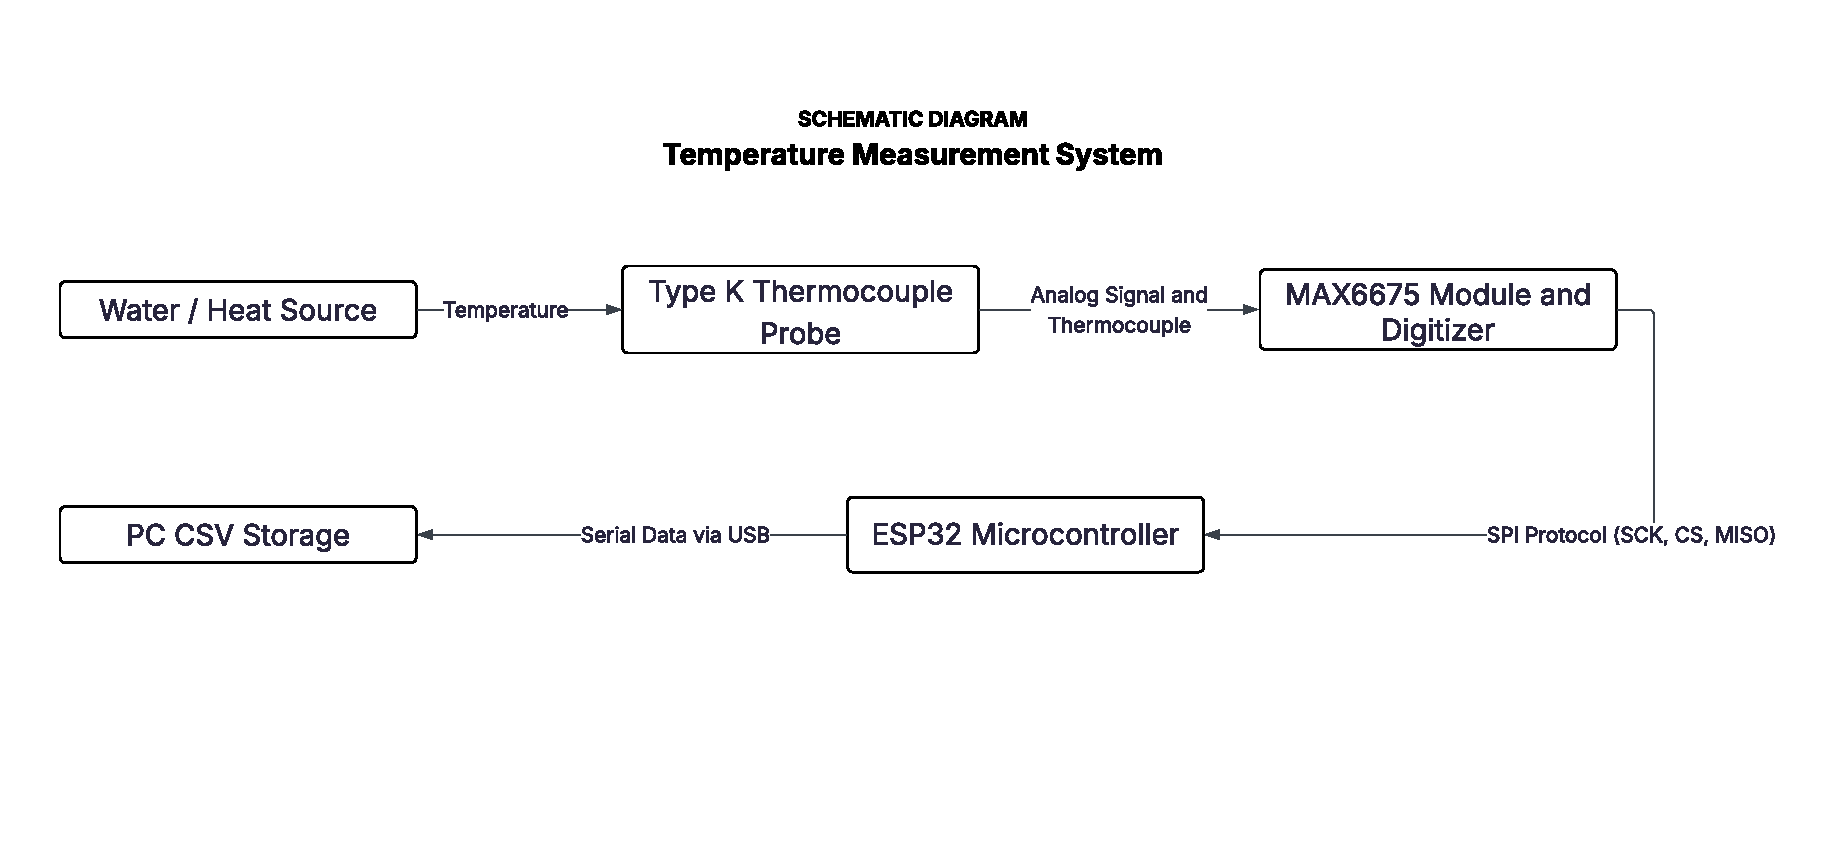
\includegraphics[width=0.95\textwidth]{diagrama_esquematico.pdf}
    \caption{Diagrama esquemático del sistema de medición de temperatura.}
    \label{fig:esquematico}
\end{figure}

Por otro lado, la captura de datos se rige por un script en Python estructurado de manera modular. El programa principal solicita la confirmación de la fase experimental e invoca la subrutina de lectura. Esta rutina toma 10 muestras estables, calcula la varianza y retorna el lote de datos estructurado para ser exportado, tal como se detalla en la Figura \ref{fig:flujo}.

\begin{figure}[H]
    \centering
    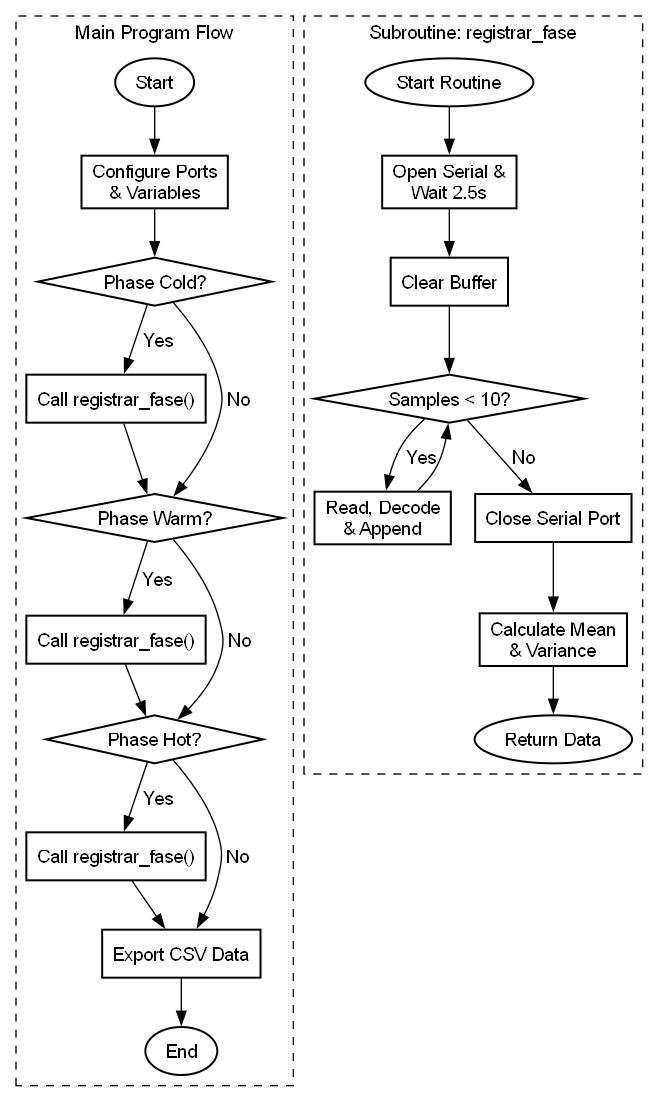
\includegraphics[width=0.75\textwidth]{diagrama_flujo.png}
    \caption{Diagrama de flujo del software de adquisición y registro CSV.}
    \label{fig:flujo}
\end{figure}

% --- F. RESULTADOS ---
\section*{F. Resultados}
\addcontentsline{toc}{section}{F. Resultados}
El sistema se ejecutó exitosamente a través de la terminal de comandos. La comunicación serial se estableció sin pérdida de paquetes, logrando registrar las muestras correspondientes a las fases térmicas definidas. El algoritmo calculó correctamente la media y la varianza para cada bloque de 10 muestras, demostrando la estabilidad de la lectura. Finalmente, el programa exportó el total de las lecturas a un archivo estructurado de forma tabular, cumpliendo con los requisitos para la etapa de análisis de datos.

% --- G. CONCLUSIONES ---
\section*{G. Conclusiones}
\addcontentsline{toc}{section}{G. Conclusiones}
La integración de hardware de bajo costo con un entorno de programación de alto nivel como Python resultó en una herramienta robusta para el diseño experimental. El uso del protocolo SPI garantizó una lectura digital libre del ruido eléctrico típico de las conversiones analógicas directas. Asimismo, la estructuración del código en subrutinas permitió mantener un control estricto sobre el tamaño de las muestras y la automatización de la bitácora en formato CSV, eliminando el error humano en la transcripción de datos.

% --- H. REFERENCIAS ---
\section*{H. Referencias}
\addcontentsline{toc}{section}{H. Referencias}
\begin{itemize}
    \item Maxim Integrated. (2002). \textit{MAX6675: Cold-Junction-Compensated K-Thermocouple-to-Digital Converter}. Datasheet.
    \item Espressif Systems. (2023). \textit{ESP32 Technical Reference Manual}. 
\end{itemize}

% Actualización de metadatos

\end{document}